 % options:
% thesis=B bachelor's thesis
% thesis=M master's thesis
% czech thesis in Czech language
% slovak thesis in Slovak language
% english thesis in English language
% hidelinks remove colour boxes around hyperlinks

\documentclass[thesis=M,czech]{FITthesis}[2012/06/26]

\usepackage[utf8]{inputenc} % LaTeX source encoded as UTF-8

\usepackage{graphicx} %graphics files inclusion
% \usepackage{amsmath} %advanced maths
% \usepackage{amssymb} %additional math symbols

\usepackage{dirtree} %directory tree visualisation

\usepackage{nameref}
\usepackage{hyperref}
\usepackage{longtable}
\usepackage{pifont}

% % list of acronyms
% \usepackage[acronym,nonumberlist,toc,numberedsection=autolabel]{glossaries}
% \iflanguage{czech}{\renewcommand*{\acronymname}{Seznam pou{\v z}it{\' y}ch zkratek}}{}
% \makeglossaries

\newcommand{\tg}{\mathop{\mathrm{tg}}} %cesky tangens
\newcommand{\cotg}{\mathop{\mathrm{cotg}}} %cesky cotangens

% % % % % % % % % % % % % % % % % % % % % % % % % % % % % % 
% ODTUD DAL VSE ZMENTE
% % % % % % % % % % % % % % % % % % % % % % % % % % % % % % 

\department{Katedra softwarového inženýrství}
\title{Letecké záznamy pro iOS pomocí moderních architektur a FRP}
\authorGN{Martin} %(křestní) jméno (jména) autora
\authorFN{Žid} %příjmení autora
\authorWithDegrees{Bc. Martin Žid} %jméno autora včetně současných akademických titulů
\author{Martin Žid} %jméno autora bez akademických titulů
\supervisor{Ing. Dominik Veselý}

\acknowledgements{Doplňte, máte-li komu a za co děkovat. V~opačném případě úplně odstraňte tento příkaz.}

\abstractCS{
%TOTO NENI FINALNI VERZE
Tato práce realizuje iOS aplikaci pro evidenci letů.  V první části analyzuji obdobné aplikace a předpisy pro piloty České republiky, podle nichž probíhá návrh funkcionality vytvářené aplikace. Podle návrhu je následně zvolena vhodná architektura a vytvořeno uživatelského rozhraní v podobě wireframů.

Aplikace je implementována s použitím zvolené architektury a pomocí principů FRP. V průběhu implementace aplikace jsou realizovány jednotkové testy a na konci jsou provedeny uživatelské testy. Na základě výsledků testů je aplikace upravena do finální podoby.

V poslední části práce popisuji výhody a nevýhody, které přinesly postupy FRP. Také hodnotím časovou a implementační náročnost oproti standardním postupům a architektuře MVC. 

V~práci jsem vytvořil funkční iOS aplikaci s využitím moderní architektury a principů FRP. Aplikace bude sloužit pilotům České republiky pro elektronickou evidenci letů a bude jim také ulehčovat administrativu s evidencí spojenou.

V~příloze této diplomové práce je možné nalézt všechny zdrojové kódy jak aplikace, tak i testů společně s~vytvořenými wireframy.
}

\abstractEN{Sem doplňte ekvivalent abstraktu Vaší práce v~angličtině.}

\placeForDeclarationOfAuthenticity{V~Praze}
\declarationOfAuthenticityOption{4} %volba Prohlášení (číslo 1-6)
\keywordsCS{mobilní aplikace pro evidenci letů, iOS, Swift, FRP, ReactiveCocoa, MVVM architektura}
\keywordsEN{flight records mobile application, iOS, Swift, FRP, ReactiveCocoa, MVVM architecture}

\begin{document}

% \newacronym{CVUT}{{\v C}VUT}{{\v C}esk{\' e} vysok{\' e} u{\v c}en{\' i} technick{\' e} v Praze}
% \newacronym{FIT}{FIT}{Fakulta informa{\v c}n{\' i}ch technologi{\' i}}

\begin{introduction}
V dnešní době, kdy existují mobilní aplikace na téměř vše, mě zarazil fakt, že u pilotů tomu tak nemusí být. Aplikace na evidenci letů samozřejmě existují, však je tu hned několik problémů. Tyto aplikace jsou často velice drahé, nemusí odpovídat leteckým přepisům České republiky nebo nemají vyhovující funkcionalitu.

Z tohoto důvodu jsem se rozhodl vytvořit iOS aplikaci na evidenci letů. Tato aplikace bude pomáhat pilotům zaznamenávat elektronicky své lety, bude také kontrolovat předpisy a umožňovat export do formátu pro tisk.

Začínám analýzou podobných aplikací, a to pro zařízení iOS i Android. Poté navrhuji vhodnou funkcionalitu a vytvářím návrh uživatelského rozhraní.

Dalším tématem, které ve své práci řeším, jsou softwarové architektury při vývoji iOS aplikace. Zde analyzuji alternativy k architektuře MVC ve spojení s funkcionálně reaktivním programováním neboli FRP.

Tuto analýzu následně aplikuji v praxi, kdy se zvolenou architekturou a FRP implementuji společně s jednotkovými testy dříve zmíněnou aplikaci. Nakonec aplikaci podrobím uživatelským testům a podle jejich výsledků
upravím aplikaci do finální podoby.

V poslední části své práce se snažím zhodnotit postupy FRP společně se mnou zvolenou moderní architekturou a jejich časovou a implementační náročnost oproti klasickému MVC.
\end{introduction}

\chapter{Cíl práce}
Cílem této práce je navrhnout a implementovat aplikaci k evidenci letů pro platformu iOS, a to pomocí postupů FRP (funkcionálně reaktivního programování) a s využitím moderní softwarové architektury jako např. MVVM nebo VIPER.  Tato aplikace bude sloužit pilotům České republiky k elektronické evidenci letů. Tento cíl je rozdělen do několika podúkolů.

V první části analyzuji podobné aplikace pro evidenci letů, a to jak pro platformu iOS, tak i pro Android. Na základě této analýzy navrhnu vhodnou funkcionalitu pro vytvářenou aplikaci. Podle navržených funkcionalit si zvolím architekturu  a navrhnu uživatelské rozhraní v podobě wireframů.

V dalším kroku aplikaci implementuji pomocí postupů FRP a se zvolenou architekturou. V průběhu realizace aplikace budou vytvářeny také testy a dokumentace aplikace.

Dále bude aplikace podrobena uživatelským testům, podle kterých bude vhodně upravena.

V poslední části budu popisovat výhody a nevýhody, které přinesly postupy FRP. Budu také hodnotit časovou a implementační náročnost oproti standardním postupům a architektuře MVC. 


\chapter{Tvorba iOS aplikací}

\section{Možnosti vývoje}
Vývoj iOS aplikace je možný hned několika způsoby, každý má své výhody a nevýhody, právě ty bych rád v této kapitole rozebral. Mezi možné způsoby vývoje bych rád zmínil nativní aplikace, hybridní aplikace a mobilní webové aplikace.

\subsection{Nativní aplikace}
Nativní aplikace jsou vyvíjeny specificky pro jednu platformu. Díky tomu mají přístup ke všem funkcím daného zařízení jako např. GPS, kamera nebo kontakty. Mohou fungovat i pouze offline, tedy bez nutnosti internetového připojení. \cite{Nielsen}

Však pokud bychom chtěli aplikaci distribuovat na více platforem, tak s tímto přístup by bylo nutné vytvořit pro každou platformu vlastní aplikaci. To by prodloužilo vývoj a znesnadnilo následnou údržbu aplikací.

Co se týče iOS vývoje, je možné si zvolit z dvou programovacích jazyků -- Objective-C nebo Swift. \cite{objc} \cite{swift}

\subsection{Hybridní aplikace}
Hybridní aplikace jsou aplikace tvořené nejčastěji pomocí HTML5 a JavaScriptu, následně jsou spuštěné v nativním kontejneru. \cite{saleforce} Jako příklad je možné uvést např. Apache Cordova. Tento kontejner umožňuje přístup k funkcím daného přístroje, podporuje použití aplikace offline a dává možnost publikace vytvořené aplikace do obchodu tzv. app store. \cite{cordova}

Však výhodou nativních aplikacím proti hybridním je to, že jsou vytvářeny přesně pro danou platformu, a tudíž jejich vzhled a výkon bude vždy lepší. \cite{upwork}

\subsection{Mobilní webové aplikace}
Poslední možností jsou mobilní webové aplikace. Tyto aplikace jsou pouze upravené webové stránky do podoby a chování nativních aplikací. Přestože běží pouze v prohlížeči, mohou mít i tyto aplikace přístup k určitým (ne však ke všem) nativním funkcím. \cite{Nielsen}

Tím, že jsou mobilní webové aplikace spouštěny v prohlížeči a nejsou stahovány přes obchody, je ulehčena údržba a vývoj, protože si uživatel nemusí vždy stahovat novou verzi aplikace.

Však tento postup má i své nevýhody. Jak již bylo zmíněno dříve, aplikace nemá přístup ke všem nativním funkcím daného přístroje. S dalším problémem se můžeme setkat u offline ukládání dat, a to se zabezpečením, které nemusí být tak dokonalé nebo uživatelsky přívětivé, jako u nativních aplikací.  \cite{saleforce}

\subsection{Zvolené řešení}
Pro svou práci jsem si zvolil možnost nativní mobilní aplikace z důvodu zaměření pouze na platformu iOS. Bude se tedy jednat pouze o jednu aplikaci, která bude moci využít všech nativních funkcionalit, výkonu i vzhledu.

\section{Architektury při tvorbě iOS aplikací}
Při tvorbě iOS aplikace je možné si vybrat z několika architektur. V této kapitole budu rozebírat pouze MVC, MVVM a VIPER.

\subsection{MVC}
Architektura MVC je zkratka pro \uv{Model View Controller} neboli tři komponenty, ze kterých se architektura skládá. Jedná se o softwarovou architekturu, které se velice často používá při tvorbě aplikací s uživatelským rozhraním. \cite{MVCMozilla}
\begin{itemize}
\item $Model$ definuje jaká data aplikace obsahuje, a pokud dojde k jakékoliv změně, tak informuje buď $Controller$ nebo $View$ (tzv. své observery). \cite{MVCGoogle}
\item $View$ vrstva je prezentována samotnému uživateli. Tedy jsou zde zobrazena aplikační data a je zachycována uživatelova práce s aplikací.\cite{MVCMozilla}
\item $Controller$ je vrstva mezi $View$ a $Model$ zabezpečující logiku aplikace. Stará se o promítnutí změn do $View$ pokud se změní $Model$. Zároveň provádí úpravy v $Model$ při uživatelově manipulaci s $View$.  \cite{MVCGoogle}
\end{itemize}

Však co se týče iOS vývoje, vrstvy $View$ a $Controller$ jsou téměř spojeny, protože $Controller$ je příliš úzce zapojený do životního cyklu $View$, což následně způsobuje velký nárůst $Controller$.\cite{Orlov}

Základní myšlenku MVC a MVC při vývoji iOS aplikace ukazují obrázky \ref{fig:mvc} (převzato a přeloženo z originálu \cite{mvc-pic}) a \ref{fig:mvc-apple} (převzato a přeloženo z originálu \cite{mvc-apple-pic}).

MVC je základní architekturou pro tvorbu iOS aplikací. Není však jedinou možností.

\begin{figure}[h]\centering
 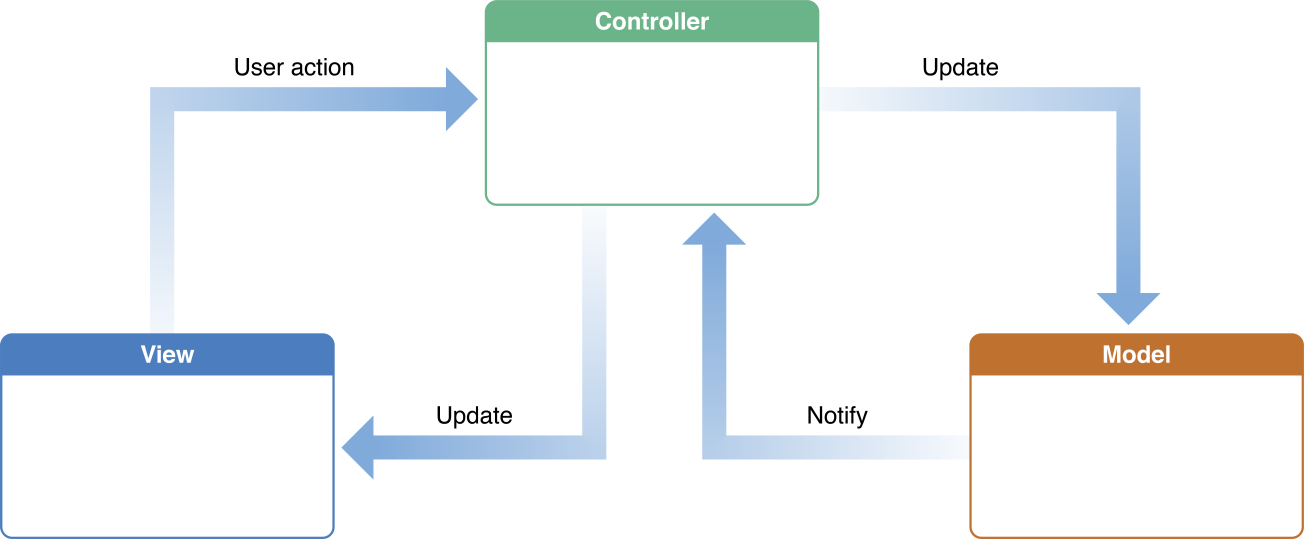
\includegraphics[width=0.99\textwidth]{./pictures/architektury/model_view_controller}
 \caption[Model-View-Controller diagram]{Model-View-Controller diagram}\label{fig:mvc}
\end{figure}

\begin{figure}[h]\centering
 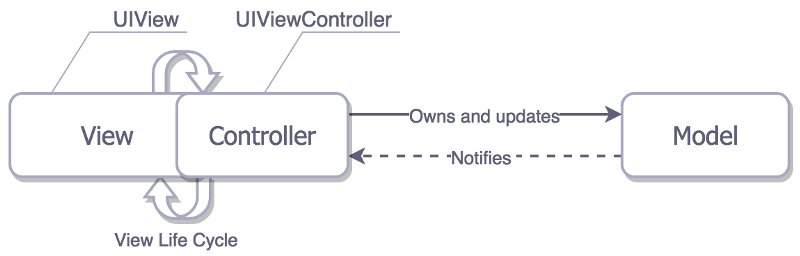
\includegraphics[width=0.99\textwidth]{./pictures/architektury/appleMVC}
 \caption[Model-View-Controller při vývoji iOS aplikace]{Model-View-Controller při vývoji iOS aplikace}\label{fig:mvc-apple}
\end{figure}

\subsection{MVVM}
Architektura MVVM má obdobné koncepce jako MVC. Jedná se také o zkratku, tentokrát \uv{Model-View-ViewModel}. \cite{MVVMMicrosoft}
\begin{itemize}
\item $Model$ je totožný s $Model$ vrstvou architektury MVC, jedná se tedy o datovou část aplikace.
\item $View$ prezentuje aplikační data uživateli a monitoruje jeho akce. Však, jak již bylo zmíněno dříve, u iOS aplikací se jedná spíše o vrstvu\\ $View/View$ $controller$. Tato vrstva obsahuje pouze minimum logiky aplikace a reaguje hlavně na $ViewModel$.  \cite{Morrison}
\item $ViewModel$ spojuje $View$ a $Model$ a zajišťuje hlavní logiku aplikace. $ViewModel$ tedy komunikuje s  $Model$ a jeho metodami a následně připravuje data pro $View$. Obsahuje také implementaci funkcí, které reagují a zpracovávají akce uživatele např.: kliknutí na tlačítko. \cite{MVVMMicrosoft}
\end{itemize}

Tedy pro shrnutí rozdílů MVC a MVVM u iOS bych zmínil to, že iOS MVC má ve výsledku téměř jen dvě vrstvy $View/View$ $controller$ a $Model$. Když potom uvažujeme architekturu MVVM ,$View/View$ $controller$  je opravdu pouze jednou vrstvou a mezi ní a $Model$ je vložena nová vrstva  $ViewModel$, která je spojuje, a do které je přesunuta i většina aplikační logiky.

Mezi výhody architektury MVVM oproti MVC patří např.:
\begin{itemize}
\item poskytuje návrhový princip tzv. separation of concerns, neboli oddělení zájmů;
\item zlepšuje možnost testovatelnosti aplikace.
\end{itemize}

Architekturu MVVM zobrazuje obrázek \ref{fig:mvvm} (převzato a přeloženo z originálu \cite{mvvm-pic}).

\begin{figure}[h]\centering
 \includegraphics[width=0.99\textwidth]{./pictures/architektury/MVVM}
 \caption[Model-View-ViewModel architektura]{Model-View-ViewModel architektura}\label{fig:mvvm}
\end{figure}

\subsection{VIPER}
VIPER je poslední rozebíranou možností, co se týče architektur. I zde je název složen z prvních písmen jednotlivých vrstev architektury, tedy \uv{View, Interactor, Presenter, Entity, Router}.
\begin{itemize}
\item $View$  zobrazuje data uživateli a předává uživatelovi vstupy vrstvě $Presenter$.
\item $Interactor$ obsahuje logiku aplikace spojenou s daty ($Entity$).
\item $Presenter$ vrstva má na starosti $View$ logiku.  Reaguje tedy na uživatelovy akce a komunikuje s vrstvou $Interactor$, od ní také přijímá nová data. \cite{Orlov}
\item $Entity$ jsou datové objekty aplikace přístupné pouze části $Interactor$.
\item $Routing$ obsahuje navigační logiku. \cite{VIPER}
\end{itemize}

Mezi výhody architektury VIPER znovu patří např.:
\begin{itemize}
\item dobře rozděluje odpovědnosti;
\item zlepšuje možnost testovatelnosti aplikace. \cite{Orlov}
\end{itemize}

Tato architektura však může být zbytečně složitá pro menší aplikace. \cite{Orlov}

Architekturu VIPER zobrazuje obrázek \ref{fig:viper} (převzato a přeloženo z originálu \cite{viper-pic}).

\begin{figure}[h]\centering
 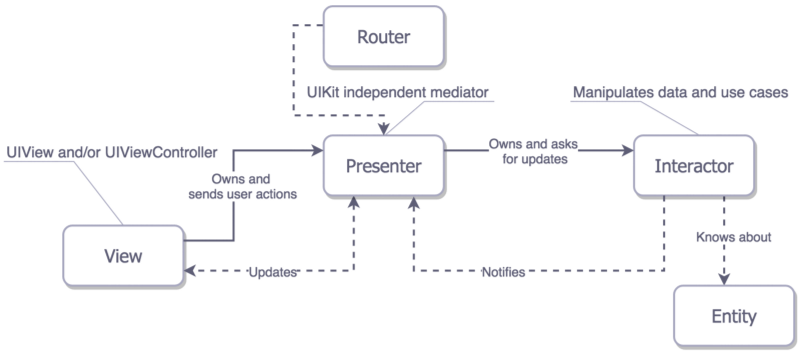
\includegraphics[width=0.99\textwidth]{./pictures/architektury/viper.png}
 \caption[VIPER architektura]{VIPER architektura}\label{fig:viper}
\end{figure}

\section{Funkcionálně reaktivní programování}
Funkcionálně reaktivní programování je kombinací funkcionálního a reaktivního programování, díky němuž dokáže aplikace dynamicky měnit stav a chování v závislosti na událostech přicházejících za daný čas. \cite{nayebi2016swift}

Pro vysvětlení, co je reaktivní programování cituji André Staltze: \uv{reaktivní programování je programování s asynchronními datovými toky}. \cite{Ztaltz2014}

Na spojení funkcionální a reaktivního programování může dívat i jako na návrhový vzor $observer$. \cite{Blackheath2016} Pozorujeme tedy např. určité vstupní pole, tlačítko nebo i dotaz na server a jsme informování o každé změně v podobě asynchronního datového toku. Na tyto datové toky je možné aplikovat funkcionální programování. Je tedy možné toky:
\begin{itemize}
\item spojovat ($merge$),
\item filtrovat ($filter$) např. pouze události, které nás zajímají,
\item mapovat ($map$) jeden tok na nový, a další. \cite{Ztaltz2014}
\end{itemize}

\subsection{FRP frameworky pro iOS}
V této kapitole jsou pouze rozebrány základy jednotlivých frameworků, podrobnější vysvětlení (zvoleného frameworku) společně s ukázkami jsou k nalezení v kapitole \nameref{chap:realizace}.

\subsubsection{ReactiveSwift}
ReactiveSwift je prvním frameworkem pro iOS podporující FRP. Obsahuje řadu základních prvků ($Signal$, $SignalProducer$, $Property$, $Action$\ldots) a operátorů podporujících myšlenku \uv{tok hodnot za čas}. \cite{ReactiveSwift}

\subsubsection{ReactiveCocoa}
ReactiveCocoa je další z FRP frameworků pro iOS. ReactiveCocoa rozšiřuje různé aspekty Apple Cocoa frameworku základními prvky frameworku ReactiveSwift. Umožňuje vazbu na prvky uživatelského rozhraní, u interaktivních prvků napojuje $Signal$ a $Action$ pro kontrolu událostí a změn. Dále také umožňuje vytvářet signály na volání metod (např. i pro UIKit třídy). \cite{ReactiveCocoa}

\subsubsection{RxSwift}
RxSwift je Swift verzí knihovny Reactive Extensions (Rx). \cite{RxSwift} Tato knihovna umožňuje vytvářet aplikace založené na událostech a asynchronních datových tocích pomocí tzv. Observables. \cite{RxNET} I přesto, že RxSwift není striktně FRP frameworkem, \cite{ReactiveExtensionsDocs} je zde uváděn, a to z důvodu velkého využití knihovny Reactive Extensions i na jiných platformách např.: JavaScript, C\#, Python. \cite{ReactiveExtensions}

\section{Perzistence dat}
Perzistence dat, neboli jejich uchování a uložení, je velice důležitou funkcionalitou většiny aplikací. V této kapitole jsou rozebírány tři možnosti zajišťující perzistenci dat iOS aplikací -- Core Data, iCloud a Realm.

\subsection{Core Data}
Core Data je Apple framework, který má na starosti model vrstvu aplikace. Stará se o životní cyklus objektů, jejich vztahy (objektový graf) i perzistenci. \cite{coredata}

Core Data má více možností na způsob uložení např. SQLite a XML. Jedná se tedy o uložení dat na disku daného zařízení.  \cite{CoreDataPersistentTypes}

Výhodou tohoto frameworku je to, že je zcela zdarma a má podporu přímo v Xcode. \cite{CoreDataXcode}

\subsection{iCloud}
iCloud je cloudové úložiště od společnosti Apple. Umožňuje ukládat aplikační data i dokumenty a přistupovat k nim na všech Apple zařízeních a na webu. \cite{iCloud}

Při vývoji iOS aplikací se pro využití iCloud používá framework CloudKit. CloudKit zajišťuje rozhraní pro komunikaci dané aplikace a iCloud. \cite{CloudKitDoc} Poskytuje ověření uživatele, tři druhy databáze -- soukromou, veřejnou a sdílenou, dále také analytický nástroj CloudKit Dashboard, který umožňuje prozkoumání dat, měření aktivity uživatelů a další. \cite{CloudKit}

CloudKit je dostupný pro členy Apple Developer programu. \cite{AppleDeveloperProgram} Tento program stojí ročně v přepočtu 2150 Kč. \cite{AppleDeveloperProgramPrice} 

\subsection{Realm}
Realm, s oficiální stránkou \url{https://realm.io}, je multiplatformní mobilní databáze, která je připravená pro jazyky Java (Android), Swift, Objective-C, JavaScript a Xamarin. Hlavní myšlenkou je kontejner objektů tzv. Realm. V těchto kontejnerech jsou uložena data, na které je možné se dotazovat, tyto data filtrovat a podobně. Na rozdíl od klasických např. SQL databází, zde pracujeme přímo s \uv{živými} objekty, tedy pokud provedeme změnu není nutné ukládat změněný objekt do databáze, ale změna se provede automaticky.

Realm je rozdělený na dvě části -- mobilní databáze Realm (Realm Mobile Database) a objektový server Realm (Realm Object Server). Jak je již z názvů možné usuzovat mobilní databáze je pouze na mobilním zařízení, jedná se tedy o offline uložení dat. Pokud však chceme data např. sdílet na více zařízení, je možné se připojit na objektový server Realm a s tím se synchronizovat. Realm se řídí strategii \uv{nejprve offine} -- čtení a zápis probíhá nejprve lokálně a až poté probíhá synchronizace se serverem.

Jedna aplikace může využívat hned několik Realm kontejnerů, a to jak lokální, tak i vzdálené, kde každý z nich může mít různá oprávnění pro různé uživatele.

Realm Mobile Database je open source, tedy zdarma. \cite{realmOverview}

\chapter{Analýza evidence letů}
\section{EASA}
EASA, neboli European Aviation Safety Agency, je agentura spadající pod Evropskou Unii, která má na starosti technické přepisy, bezpečnost, regulace a certifikace v oboru letectví. \cite{EU} 

Pro tuto diplomovou práci je EASA důležitá, protože vydává i pokyny např. pro evidenci letů nebo limity odlétaných hodin. \cite{EASARegulations}

\subsection{Pokyny pro evidenci letů}
Pokyny pro evidenci letů udává předpis FCL.050. Tento předpis specifikuje povinné položky každého leteckého záznamu. \cite{FCL} 

\uv{
Každý záznam letů by měl obsahovat minimálně tyto informace:
\begin{enumerate}
\item osobní informace: jméno a adresu pilota;
\item každý záznam letu by měl obsahovat:
	\begin{itemize}
	\item jméno velícího pilota (PIC -- Pilot-in-command),
	\item datum letu,
	\item čas a místo odletu a příletu,
	\item typ, značku, model, variantu a registraci letadla,
	\item označení zda je letadlo jednomotorové (SE -- single engine) nebo vícemotorové (ME -- multi engine),
	\item čas letu,
	\item celkový čas letu.
	\end{itemize}
\item každý záznam z výcvikového zařízení pro simulaci letu (FSTD -- flight simulation training devices) by měl obsahovat:
	\begin{itemize}
	\item typ a kvalifikační číslo výcvikového zařízení,
	\item instrukce výcvikového zařízení pro simulaci letu,
	\item datum,
	\item čas,
	\item celkový čas.
	\end{itemize}
\item funkce pilota -- velící pilot (včetně sólového, velícím pilotem student (Student PIC) nebo velící pilot pod dohledem (PICUS -- pilot-in-command under supervision)), druhý pilot, dvojí pilot (dual), instruktor (FI -- Flight Instructor) nebo zkoušející (FE -- Flight Examiner);
\item provozní podmínky -- pokud se let uskutečnil v noci nebo pokud byl prováděn podle pravidel pro let podle přístrojů.
\end{enumerate}
} \cite{FCL} (překlad vlastní)

\subsection{Limity}
Limity letového času a času ve službě obsahuje předpis ORO.FTL.210.

\uv{
Celková doba služby, na kterou může být člen posádky přidělen, nesmí překročit:
\begin{enumerate}
\item 60 hodin služby za 7 po sobě jdoucích dnů;
\item 110 hodin služby za 14 po sobě jdoucích dnů; a 
\item 190 hodin služby za 28 po sobě jdoucích dnů, rozdělených co nejrovnoměrněji během tohoto období.
\end{enumerate}
Celkový čas, na který je jedinec přidělen jako člen provozní posádky, nesmí překročit:
\begin{enumerate}
\item 100 hodin letu za 28 po sobě jdoucích dnů;
\item 900 hodin letu v kalendářním roce; a
\item 1000 hodin letu během 12 po sobě jdoucích kalendářních měsících.
\end{enumerate}
Poletová služba se počítá do doby služby.
} \cite{FTL} (překlad vlastní)

\subsection{Zdravotní certifikáty}
Informace o zdravotních certifikátech obsahuje předpis Part-MED. Certifikáty jsou tří druhů -- zdravotní certifikát třídy 1 (Class 1 medical certificate), zdravotní certifikát třídy 2 (Class 2 medical certificate) a zdravotní certifikát pro licence na lehká letadla (LAPL -- Light Aircraft Pilot Licence). Každý z těchto certifikátů má jinak nastavenou dobu platnosti a je pro jiné typy pilotních licencí.

LAPL certifikát je pouze pro pilotní licence na lehká letadla. Platnost je 60 měsíců u pilotů do věku 40 let, poté je platnost pouze 24 měsíců.

Zdravotní certifikát třídy 2 je pro pilotní licence PPL (Private Pilot Licence), SPL (Sailplane Pilot Licence) a BPL (Balloon Pilot Licence), tedy pro piloty soukromých letadel, kluzáků a balónů. Platnost licence se znovu odvíjí od věku pilota -- 60 měsíců u pilotů do věku 40 let, následně 24 měsíců do věku 50 let a nakonec platnost licence klesá na 12 měsíců.

Zdravotní certifikát třídy 1 je certifikát nejvyšší úrovně. Je pro pilotní licence CPL (Commercial Pilot Licence), MPL (Multi-crew Pilot Licence) a ATPL (Airline Transport Pilot Licence), tedy pro piloty komerčních, vícečlenných a dopravních letadel. Platnost licence je 12 měsíců. To neplatí u pilotů starších 40 let, létajících jednopilotní komerční lety s cestujícími nebo u pilotů starších 60 let, zde se platnost licence snižuje na 6 měsíců. \cite{CAA}

\section{Analýza existujících aplikací pro evidenci letů}
Tato kapitola se zabývá analýzou již existujících aplikací pro evidenci letů. Pro analýzu bylo vybráno pět aplikací -- tři pro iOS a dvě pro platformu Android.
\begin{enumerate}
\item LogTen Pro X -- iOS aplikace v angličtině vyvíjená společností Coradine Aviation. \cite{appStoreLogTen}
\item Logbook Pro Aviation Flight Log for Pilots -- druhá iOS aplikace, také v angličtině, vytvořená NC Software, Inc. \cite{appStoreLogbookPro}
\item Safelog Pilot Logbook -- poslední z analyzovaných iOS aplikací. I tato aplikace je v anglickém jazyce. Publikována Dauntless Software. \cite{appStoreSafeLog}
\item FlyLogio - Pilot Logbook -- česká aplikace vyvinutá pro platformu Android společností FlyLogio.com. \cite{googleFlyLogio}
\item Smart Logbook -- anglická Andriod aplikace vydána firmou Kviation, Inc. \cite{googleSmartLogbook}
\end{enumerate}

\begin{figure}[]\centering
 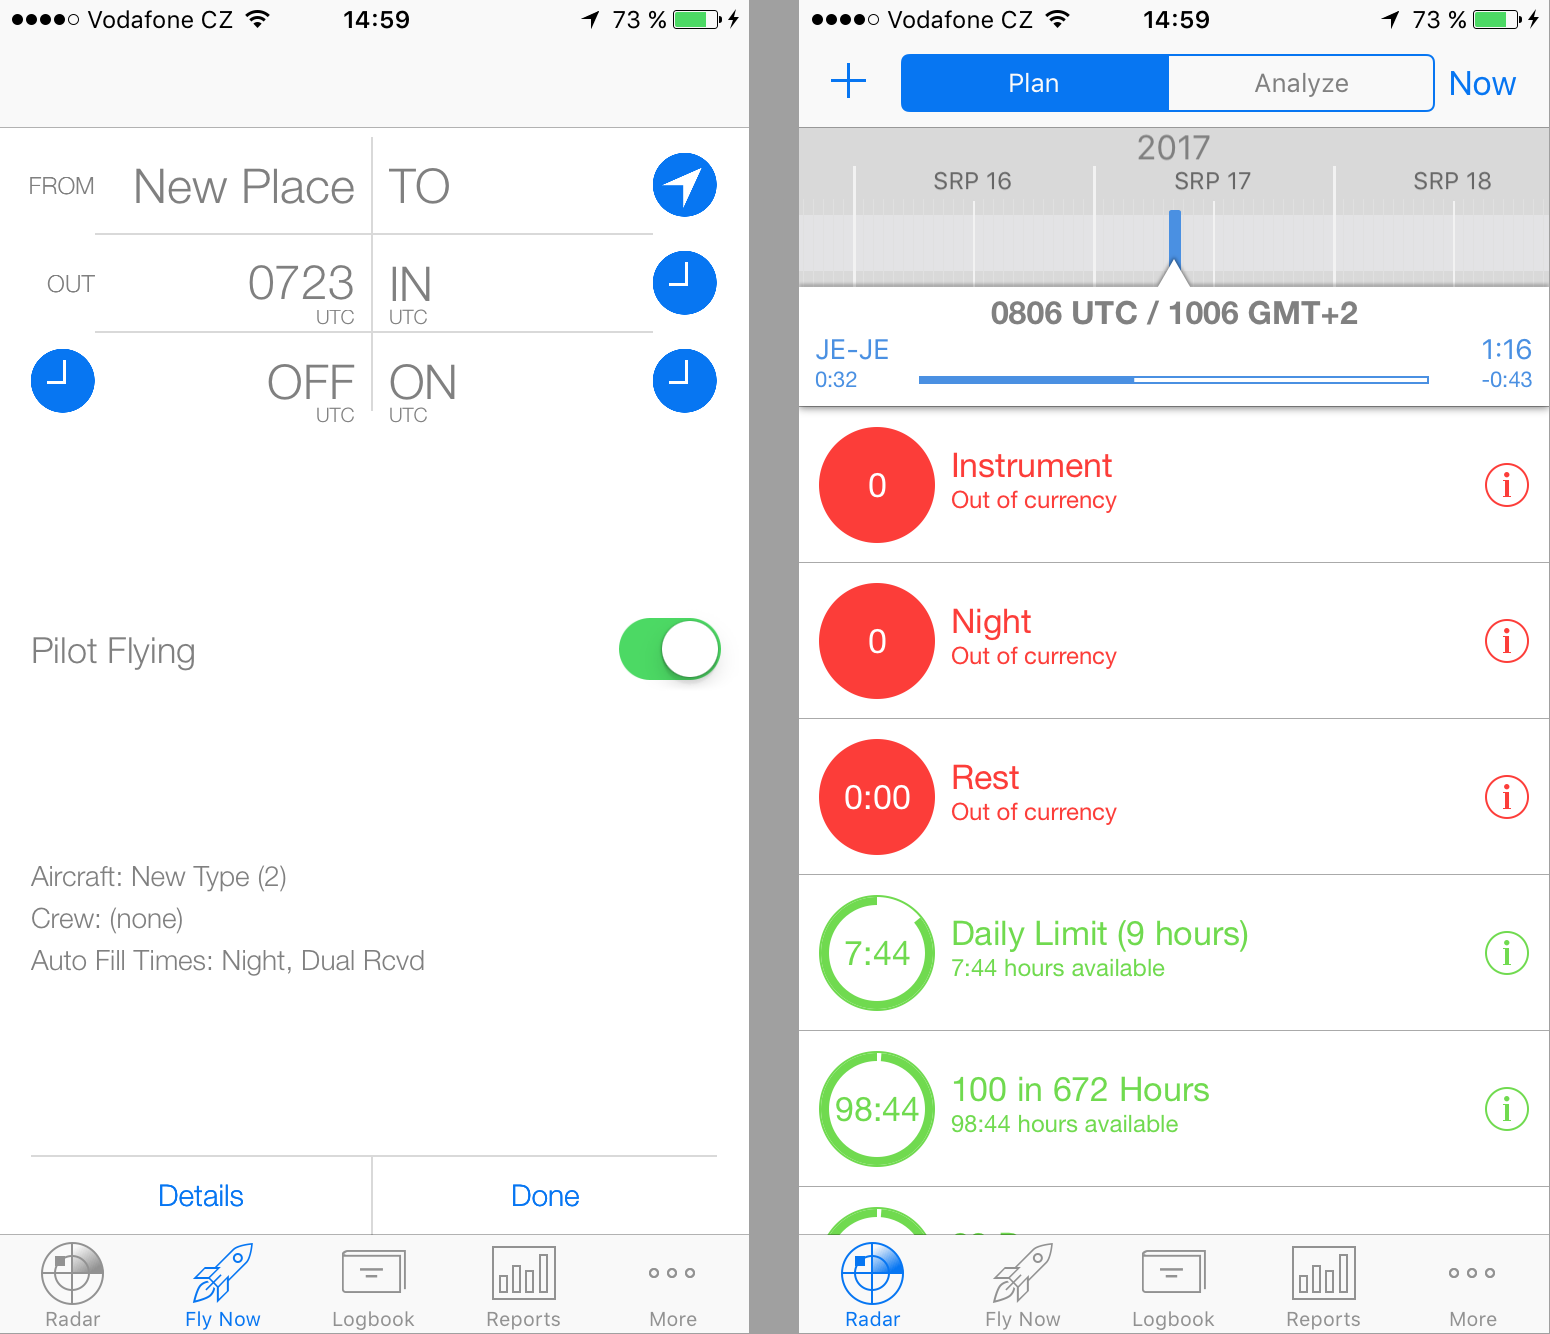
\includegraphics[width=0.99\textwidth]{./pictures/existujiciAplikace/LogTenProX}
 \caption[LogTen Pro X]{LogTen Pro X}\label{fig:LogTenProX}
\end{figure}

\begin{figure}[]\centering
 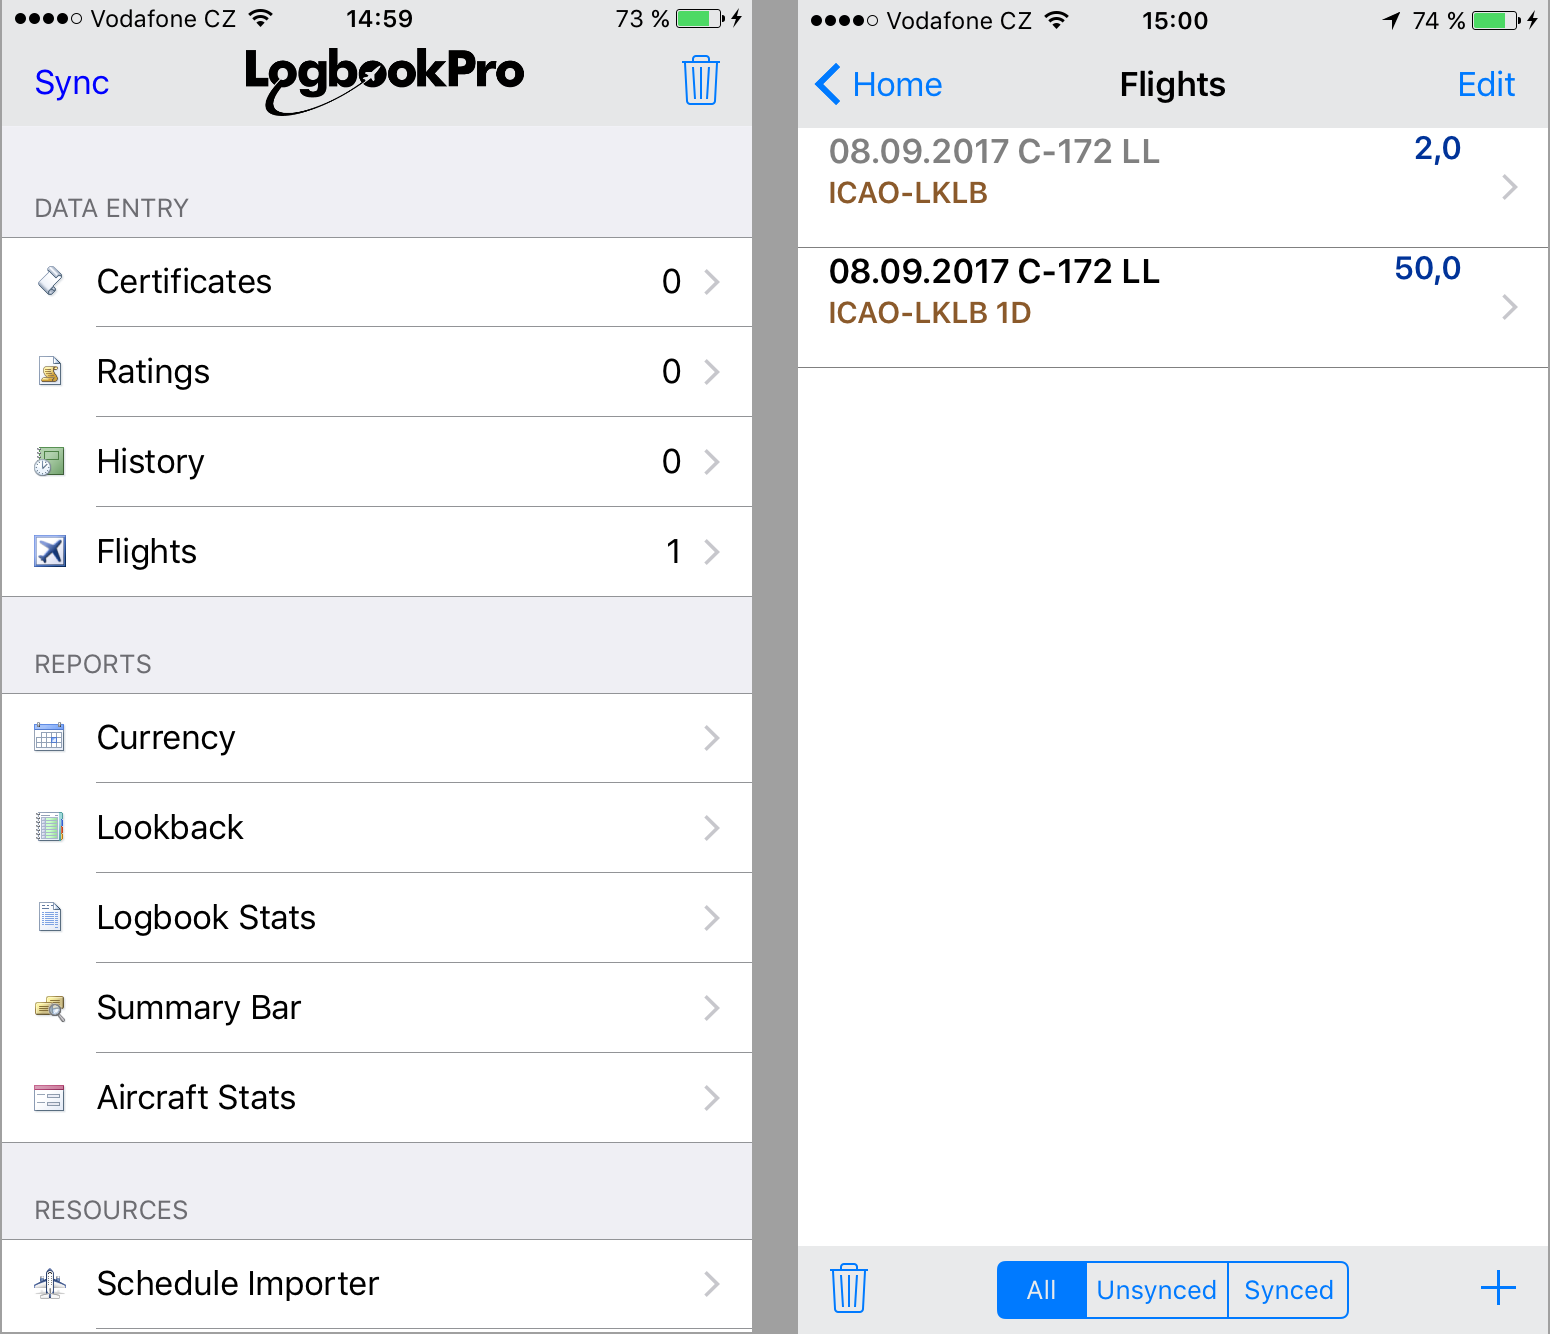
\includegraphics[width=0.99\textwidth]{./pictures/existujiciAplikace/LogbookPro}
 \caption[Logbook Pro Aviation Flight Log for Pilots]{Logbook Pro Aviation Flight Log for Pilots}\label{fig:LogbookPro}
\end{figure}

\begin{figure}[]\centering
 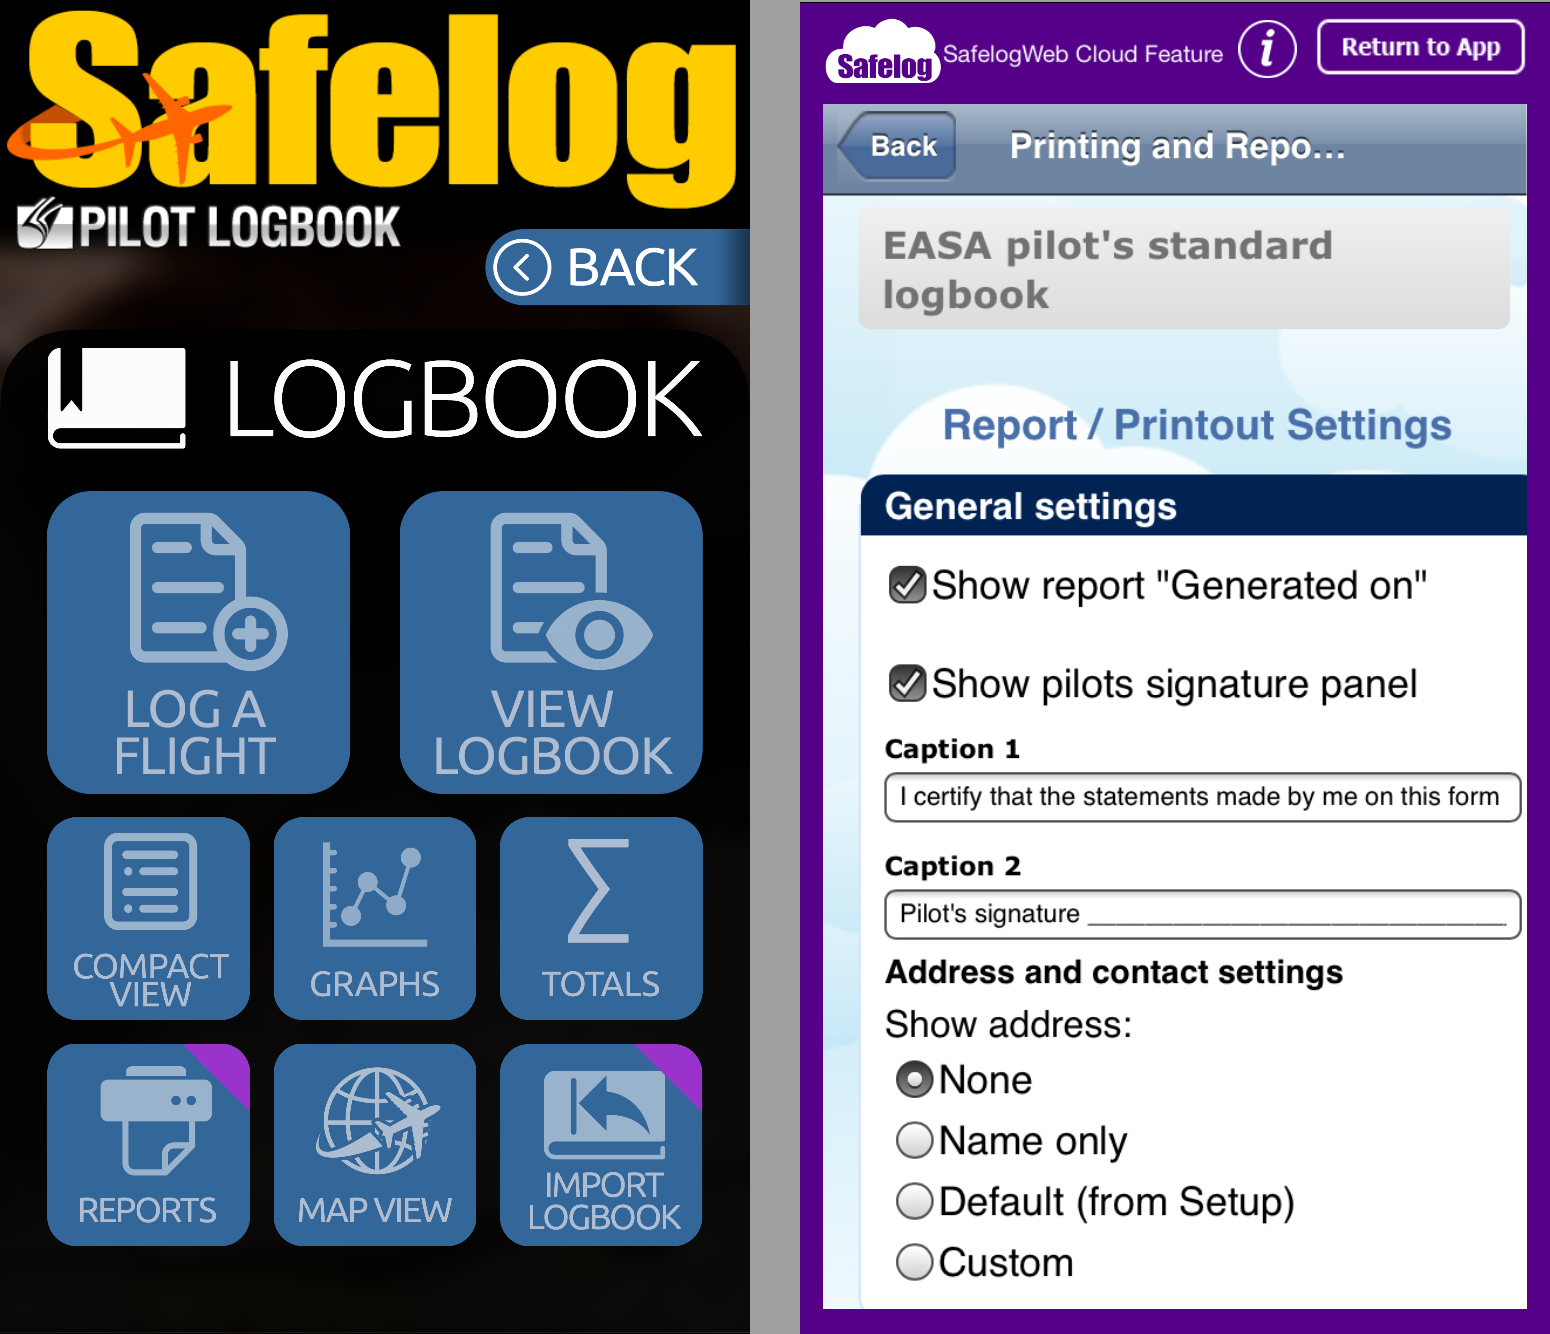
\includegraphics[width=0.99\textwidth]{./pictures/existujiciAplikace/Safelog}
 \caption[Safelog Pilot Logbook ]{Safelog Pilot Logbook }\label{fig:Safelog}
\end{figure}

\begin{figure}[]\centering
 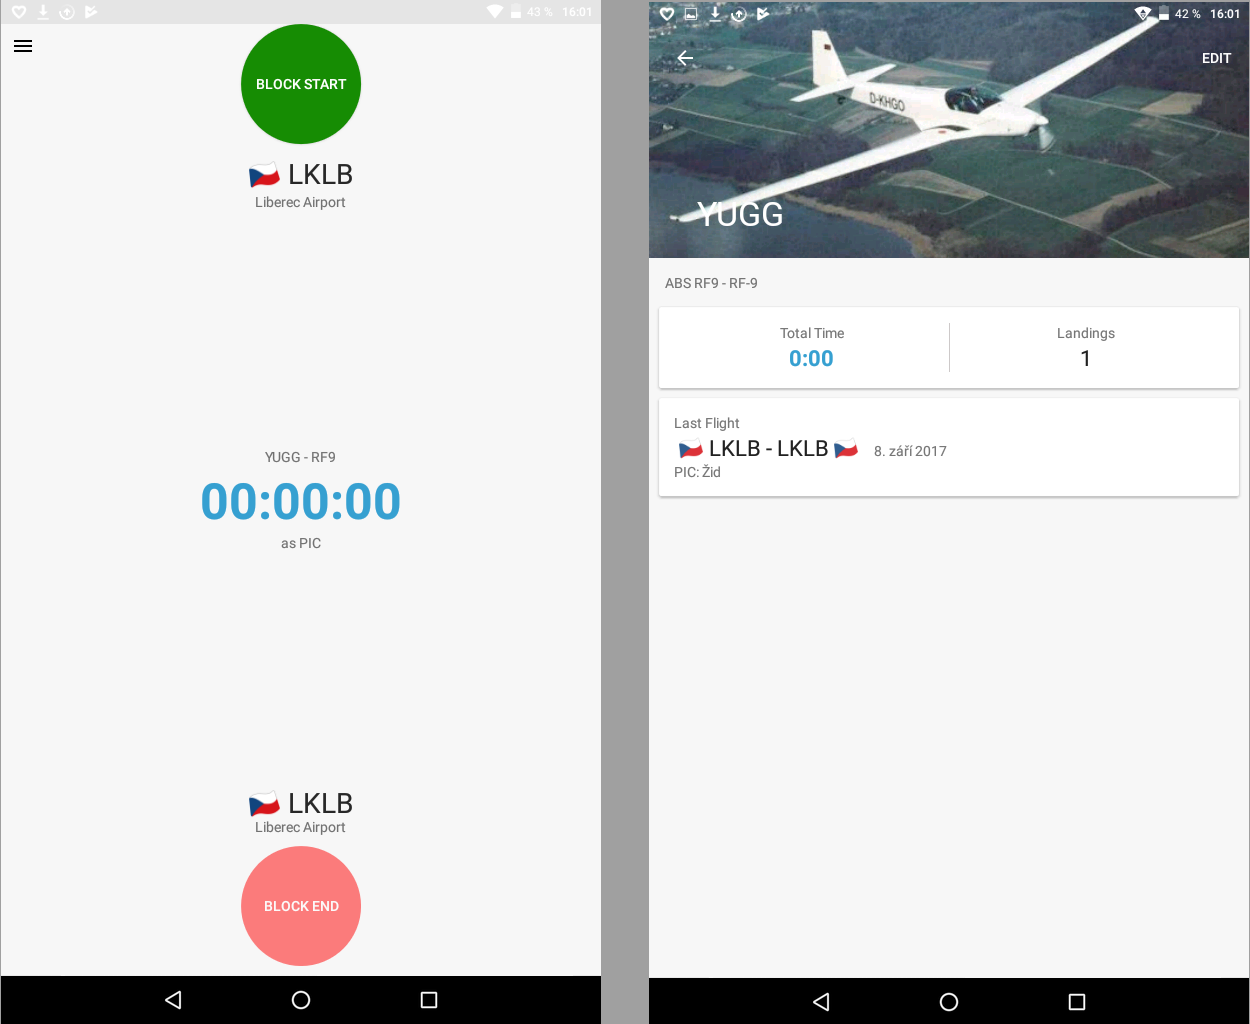
\includegraphics[width=0.99\textwidth]{./pictures/existujiciAplikace/FlyLogio}
 \caption[FlyLogio]{FlyLogio}\label{fig:FlyLogio}
\end{figure}

\begin{figure}[]\centering
 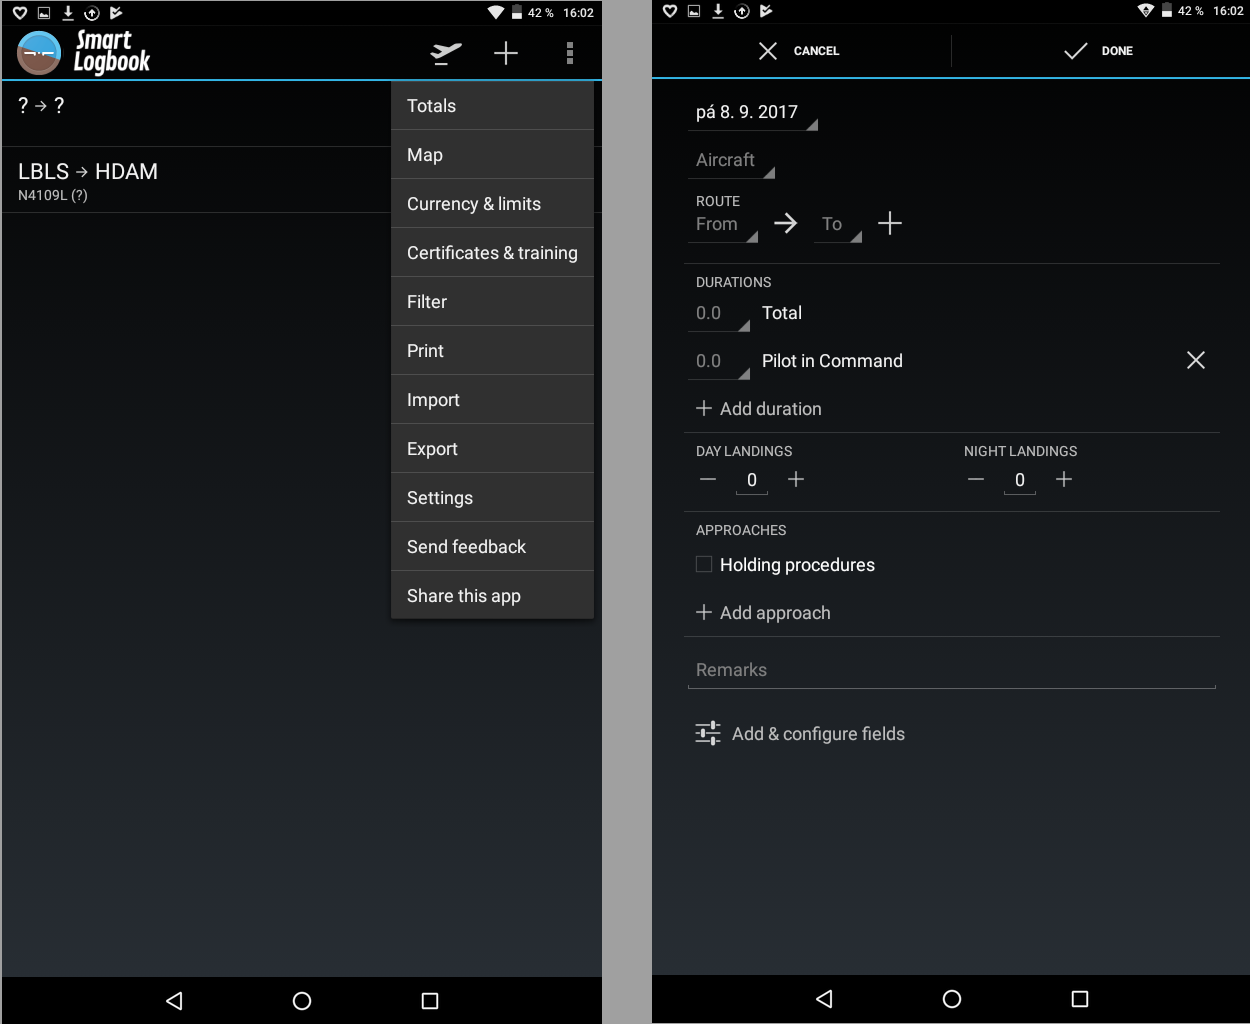
\includegraphics[width=0.99\textwidth]{./pictures/existujiciAplikace/SmartLogbook}
 \caption[Smart Logbook]{Smart Logbook}\label{fig:LogTenProX}
\end{figure}

\subsection{Kritéria hodnocení}
Kritéria hodnocení byla rozdělena do několika kategorií -- přihlášení, platby, napojení externích databází, doplňkové položky při vkládání záznamu, limity a certifikáty, reporty a zálohování.	

Při vkládání záznamu jsou brány v potaz pouze doplňkové položky, protože aplikace bude tvořena podle předpisu EASA FCL.050, který udává povinné údaje při evidování letu. Také položka v hodnocení  -- reporty podle EASA, je analyzována z pohledu předpisu FCL.050. 

Všechny položky hodnocení jsou uváděny z pohledu mobilní/tablet aplikace.

\subsection{Srovnávací tabulka}
\newcommand{\OK}{\ding{51}}
\newcommand{\NOK}{\ding{55}}
\newcommand{\rot}{\rotatebox{90}}

{\setlength\extrarowheight{2pt}
\begin{longtable}{@{\extracolsep{\fill}}l c c c c c c}
   \caption[Srovnávací tabulka]{Srovnávací tabulka}\label{tab:srovnavaci_tabulka} \\
   Kritéria & \rot{Log Ten Pro X} & \rot{Logbook Pro} & \rot{Safelog} &
   \rot{FlyLogio} & \rot{Smart Logbook} & \rot{Výsledek} \\
  \endfirsthead
   \caption[Srovnávací tabulka]{Srovnávací tabulka}\label{tab:srovnavaci_tabulka} \\
   Kritéria & \rot{Log Ten Pro X} & \rot{Logbook Pro} & \rot{Safelog} &
   \rot{FlyLogio} & \rot{Smart Logbook} & \rot{Výsledek} \\
  \endhead

   \hline
   \multicolumn{7}{c}{Přihlášení} \\
   \hline
   Aplikace funkční bez přihlášení 			 & \OK & \NOK & \NOK & \NOK & \NOK & 1/5 \\
   Možnost přihlášení								 & \OK & \OK & \OK & \OK & \OK  & 5/5 \\
   
   \hline
   \multicolumn{7}{c}{Platby} \\
   \hline
   Platby jednorázové			 & \NOK & \NOK & \NOK & \NOK & \OK & 1/5 \\
   Opakované platby			 & \OK & \OK & \OK & \OK & \OK  & 5/5 \\
   
   \hline
   \multicolumn{7}{c}{Napojení externích databází} \\
   \hline
   Napojení na databázi letišť		 & \NOK & \OK \footnote{Logbook Pro umí nalézt pouze nejbližší letiště.} & \OK & \OK & \OK & 4/5 \\
   Napojení na databázi letadel	 & \NOK & \NOK & \OK & \OK & \NOK  & 2/5 \\
   
   \hline
   \multicolumn{7}{c}{Doplňkové položky při vkládání záznamu} \\
   \hline
   Možnost přidání fotky						 & \OK & \NOK & \OK & \NOK & \NOK & 2/5 \\
   Možnost přidání dokumentu			 & \OK & \NOK & \OK & \NOK & \NOK & 2/5 \\
   
   \hline
   \multicolumn{7}{c}{Limity a certifikáty} \\
   \hline
   Kontrola limitů					 & \OK & \OK & \OK \footnote{Safelog zobrazuje limity ve webové verzi.} & \NOK & \OK & 4/5 \\
   Certifikáty							 & \OK & \OK & \OK \footnote{Safelog zobrazuje certifikáty ve webové verzi.} & \NOK & \OK & 4/5 \\
   
   \hline
   \multicolumn{7}{c}{Reporty} \\
   \hline
   Generování reportů					 & \OK & \NOK & \OK \footnote{Safelog zobrazuje reporty ve webové verzi.}  & \NOK & \OK & 3/5 \\
   Reporty podle EASA					 & \NOK & \NOK & \OK & \NOK & \OK & 2/5 \\
   Jiné reporty								 & \OK & \OK & \OK & \NOK & \OK & 2/5 \\
   
   \hline
   \multicolumn{7}{c}{Perzistence dat} \\
   \hline
   iCloud/Google					 & \OK & \NOK & \NOK & \OK & \OK & 3/5 \\
   Vlastní řešení						 & \NOK & \OK & \OK & \NOK & \NOK & 2/5 \\
   Synchronizace více zařízení  & \OK & \OK & \OK & \OK & \OK & 5/5 \\

\end{longtable}
}
\subsection{Výsledky a vlastní zhodnocení}
\subsubsection{LogTen Pro X}
LogTen Pro X je z analyzovaných iOS aplikací nejvíce uživatelsky přívětivá. Zobrazuje přehledně limity a certifikáty, i vkládání je intuitivní. Má však i několik nedostatků: 
\begin{itemize}
\item není napojená na databázi letišť, tudíž uživatel musí vyplnit všechny informace o daném letišti sám, bez automatického doplnění nebo našeptávání;
\item neumožňuje generování reportů podle předpisu EASA FCL.050;
\item aplikace je placená ročně --
	\begin{itemize}
	\item iPhone + iPad + Mac -- 3550 Kč,
	\item Mac -- 3550 Kč,
	\item iPhone + iPad -- 2150 Kč.
	\end{itemize}
\end{itemize}
Data o aplikaci a cenách jsou získány přímo z aplikace LogTen Pro X. 

\subsubsection{Logbook Pro Aviation Flight Log for Pilots}
Aplikace Logbook Pro vyžaduje pro přihlášení stažení PC aplikace (pouze pro Windows). S touto aplikací je následně synchronizován. Některá funkcionalita, např. generování reportů, je dostupná pouze v PC verzi.

PC verze aplikace je zadarmo pouze ve zkušební verzi, poté základní verze stojí v přepočtu 1800 Kč. iOS verze aplikace se platí ročně v přepočtu za 1045 Kč, je nutné si zaplatit i zálohování a další funkcionality. \cite{SafelogPrices}

\subsubsection{Safelog Pilot Logbook}
Safelog Pilot Logbook obsahuje pouze některé funkce přímo v aplikaci, u ostatních je uživatel odkázán do webového rozhraní (SafelogWeb Cloud) viz. \ref{fig:Safelog}. Toto webové rozhraní zobrazené v aplikaci však není přizpůsobené pro mobilní zařízení, často je zobrazena pouze část stránky a není možné např. vyplnit všechna pole formuláře.

Tato aplikace však, pokud budeme brát v potaz i funkce ve webovém rozhraní, obsahuje nejširší spektrum funkcionalit.

Samotná aplikace je zadarmo, ale pro plnou verzi aplikace je nutné předplatné. To se pohybuje od 1320 Kč za jeden rok až po 8990 Kč za deset let. Data o aplikaci a cenách jsou získány z aplikace Safelog Pilot Logbook.

\subsubsection{FlyLogio - Pilot Logbook}
Android aplikace FlyLogio - Pilot Logbook je jedinou aplikací kompletně zadarmo. Z uživatelského pohledu se jedná o přehlednou a jednoduchou aplikaci.  Však neobsahuje takovou funkcionalitu jako ostatní placené aplikace, např. chybí generování jakýchkoliv reportů nebo kontrolování limitů.

\subsubsection{Smart Logbook}
Smart Logbook je poslední analyzovanou aplikací, jedná se o Android aplikaci. Obsahuje mnoho funkcionalit -- generování reportů podle mnoha norem, zobrazení mapy se zaznamenáním jednotlivých letů, hlídání limitů i expirace certifikátů.

Tato aplikace je zadarmo pouze ve zkušební verzi, následně je nutné aplikaci zakoupit za 300 Kč. Je nutné také platit za zálohování a synchronizaci dat, a to buď 20 Kč za měsíc, nebo 120 Kč za rok. Informace o cenách jsou získány z aplikace Smart Logbook.

\subsubsection{Závěr analýzy}
Tato analýza posloužila při návrhu funkcionalit iOS aplikace ve formě případů užití, při návrhu uživatelského rozhraní a také při výběru vhodného nástroje na perzistenci dat.

\chapter{Návrh}

\section{Funkční a nefunkční požadavky}
\subsection{Funkční požadavky}
Funkční požadavky jsou uvedeny pouze jmenovitě. Podrobnější popis je uveden v podobě případů užití.
\begin{enumerate}
\item Evidování leteckých záznamů.
\item Vyhledávání v leteckých záznamech.
\item Kontrola limitů.
\item Evidence zdravotních certifikátů.
\item Generování reportů do formátu PDF.
\end{enumerate}
\subsection{Nefunkční požadavky}
\begin{enumerate}
\item Funkční pro iOS 11 -- aplikace bude dostupná pro verzi operačního systému iOS 11.
\item Aplikace pro iPhone a iPad -- uživatelské rozhraní bude přizpůsobeno jak telefonům, tak tabletům.
\item Stejná data na více uživatelových zařízeních -- všechna data budou zálohována online a uživatel k nim bude mít přístup na všech zařízeních s iOS 11 pod svým účtem.
\item Dostupnost dat offline -- uživatel bude mít přistup ke všem dříve staženým/vytvořeným záznamům. Aplikaci bude možné používat i bez internetového připojení, k synchronizaci dojde až ve chvíli, kdy bude internetové připojení k dispozici.
\item Aplikace podle EASA -- aplikace se bude řídit předpisy EASA a to přesně: FCL.050 u evidence letů,  ORO.FTL.210 v případě limitů a Part-MED při evidenci zdravotních certifikátů.
\end{enumerate}

\section{Navržená funkcionalita v podobě případů užití}
Případy užití (use cases) byly využity při návrhu funkcionalit iOS aplikace. Jsou obsaženy přímo v práci z důvodu přehledného zobrazení navržených funkcionalit a možnosti dovysvětlením u některých z nich.

Diagram případů užití zobrazuje obrázek \ref{fig:UC}

\begin{figure}[]\centering
 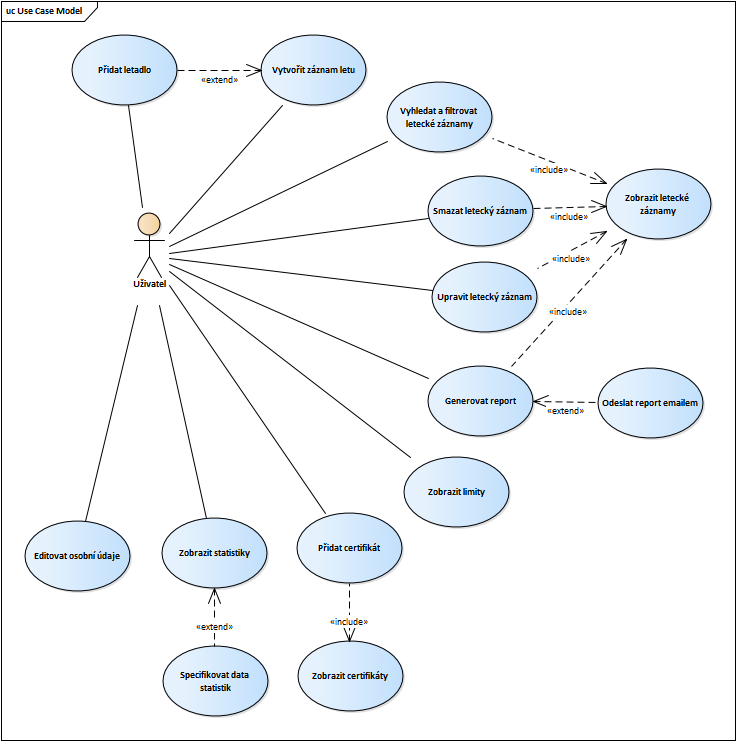
\includegraphics[width=0.99\textwidth]{./pictures/UC/UC}
 \caption[Případy užití]{Případy užití}\label{fig:UC}
\end{figure}

\subsection{Vytvořit záznam letu}
Vytvoření leteckého záznam umožňuje uživateli vložit nový záznam letu do aplikace.

Hlavní scénář --
\begin{itemize}
\item Případ užití začíná, když chce uživatel evidovat svůj let.
\item Systém zobrazí formulář umožňující zadat: jméno velícího pilota, datum letu, čas a místo odletu a příletu, letadlo, čas letu, celkový čas letu, počet vzletů a přistání, pilotovu funkci při letu a provozní podmínky.
\item Uživatel vyplní formulář.
\item Aplikace uloží informace o letu.
\end{itemize}

Alternativní scénář --
\begin{itemize}
\item Případ užití začíná, když chce uživatel evidovat záznam z výcvikového zařízení pro simulaci letu.
\item Systém zobrazí formulář umožňující zadat: typ a kvalifikační číslo výcvikového zařízení, datum a čas.
\item Případ užití pokračuje 3. krokem hlavního scénáře.
\end{itemize}

Aplikace bude napojena na databázi letišť, pro jednoduché evidování místa odletu a příletu. Nebude však napojena na databázi letadel, protože uživatel u každého letadla musí vyplnit minimálně registrační číslo. Pokud by uživatel musel letadlo najít a zeditovat, je výhodnější pokud si sám letadlo přidá. Dalším důvodem k tomu rozhodnutí je, že pilot létá velmi často pouze s jedním letadlem a proto funkcionalitu přidání letadla nebude používat příliš často.

\subsection{Přidat letadlo}
Přidání letadla dává uživateli možnost přidat letadlo, které pak může vkládat do záznamů o letu.

\begin{itemize}
\item Případ užití začíná, když chce uživatel přidat nové letadlo.
\item Systém zobrazí formulář  umožňující zadat: typ, značku model, variantu, registrační číslo letadla a zda je letadlo jednomotorové nebo vícemotorové.
\item Uživatel vyplní všechna pole formuláře.
\item Aplikace uloží letadlo.
\end{itemize}

\subsection{Zobrazit letecké záznamy}
Zobrazení leteckých záznamů zobrazuje jednotlivé záznamy v podobě tabulky, kde u každého záznamu jsou vidět základní informace. Mezi tyto informace patří: místo odletu a přílet, datum, čas letu a letadlo.

\subsection{Vyhledat a filtrovat letecké záznamy}
Tato funkcionalita umožňuje uživateli vyhledávání a filtrování leteckých záznamů.

\begin{itemize}
\item Případ užití začíná, pokud chce uživatel vyhledat nebo vyfiltrovat letecké záznamy.
\item Include (Zobrazit letecké záznamy).
\item Aplikace zobrazí formulář, který umožňuje: zadat hledaný text, nastavit zda se jedná o záznam letu nebo o záznam z výcvikového zařízení, zvolit typ letadla nebo přesné letadlo a nastavit období.
\item Uživatel vyplní pole, podle kterých chce vyhledávat/filtrovat.
\item Systém zobrazí pouze záznamy odpovídající zvoleným parametrům.
\end{itemize}

\subsection{Smazat letecký záznam}
Smazání leteckého záznamu umožňuje uživateli smazat letecký záznam, který předtím sám vytvořil.

\begin{itemize}
\item Případ užití začíná, když chce uživatel smazat jeden ze svých leteckých záznamů.
\item Include (Zobrazit letecké záznamy).
\item Uživatel si zvolí záznam, který chce smazat.
\item Aplikace zobrazí potvrzovací dialog.
\item Uživatel potvrdí smazání.
\item Aplikace odstraní položku ze seznamu.
\end{itemize}

\subsection{Upravit letecký záznam}
Upravení leteckého záznamu umožňuje uživateli upravit všechny položky zvoleného letecké záznamu.

\begin{itemize}
\item Případ užití začíná, když chce uživatel upravit letecký záznam.
\item Include (Zobrazit letecké záznamy).
\item Uživatel si zvolí záznam, který chce upravit.
\item Scénář pokračuje krokem 2 Vytvořit záznam letu.
\end{itemize}

\subsection{Zobrazit limity}
Tato funkcionalita slouží ke zobrazení limitů a kontrole zda jsou všechny limity v normě.

\subsection{Zobrazit certifikáty}
Tato funkcionalita umožňuje uživateli zobrazit všechny jeho certifikáty, společně s kontrolou platnosti a počtem dní do jejich expirace.

\subsection{Přidat certifikát}
Tato funkce umožňuje uživateli přidat certifikát a to buď dle šablony pro zdravotní certifikáty (LALP, třídy 1 a třídy 2), nebo vlastní.

\begin{itemize}
\item Případ užití začíná, když chce uživatel vytvořit nový certifikát.
\item Include (Zobrazit certifikáty).
\item Aplikace zobrazí formulář s možností vytvoření vlastního certifikátu nebo dle šablony. Ve formuláři je následně možné zadat: název certifikátu, datum vydání, datum expirace a popis.
\item Uživatel povinně vyplní název a datum expirace.
\item Aplikace uloží certifikát.
\end{itemize}

\subsection{Zobrazit statistiky}
Zobrazení statistik zobrazuje nalétané hodiny (celkově, v noci, podle přístrojů a v různých pilotových funkcích).

\subsection{Specifikovat data statistik}
Tato funkcionalita umožňuje specifikovat data, ze kterých jsou zobrazeny statistiky.
Je možné specifikovat: text, zda jsou ve statistikách zobrazeny záznamy letů a/nebo záznamy ze simulátoru, typ letadla nebo přesné letadlo a období.

\subsection{Editovat osobní údaje}
Editace osobních údajů umožňuje uživateli upravit své osobní informace. Mezi tyto informace patří: jméno a příjmení, adresa a věk.

U osobních údajů je důležitý hlavně věk, který hraje roli u zdravotních certifikátů.

\subsection{Generovat report}
Generování reportu umožňuje uživateli vygenerovat report ve formátu PDF z nímž zvolených záznamů.

\begin{itemize}
\item Případ užití začíná, jestliže se uživatel rozhodne vygenerovat report.
\item Aplikace zobrazí formulář s možným výběrem záznamů, které se v reportu objeví.
\item Uživatel si zvolí záznamy.
\item Aplikace vytvoří report ve formátu PDF se zvolenými záznamy letů.
\end{itemize}

\subsection{Odeslat report emailem}
Funkcionalita odeslání reportu emailem umožňuje uživateli, poté co vygeneroval report, odeslat tento report přes email.

\section{Návrh uživatelského rozhraní}
Návrh uživatelského rozhraní přímo navazuje na návrh funkcionalit. Pro tento návrh byl použit wireframe.

\subsection{Wireframe}
Wireframe je technika, která se používá v brzké fázi vývoje softwaru \cite{nngWireframe} pro rozvržení základních prvků obrazovek a navržení hlavních průchodů aplikací (navigace). Protože se jedná pouze o návrh, nemusí wireframe podporovat dynamicky měnící se obsah nebo např. nemusí zobrazovat chybové hlášky.

Wireframe může posloužit k první heuristické analýze a k uživatelským testům ještě před vývojem dané aplikace. \cite{exux}

Wireframe pro tuto práci byl vytvořen ve webovém nástroji NinjaMock (\url{https://ninjamock.com}). Z tohoto nástroje byl wireframe následně exportován do formátu pdf a ninjamock package. Tyto exporty jsou k nalezení v příloze této diplomové práce. 

Exportovaný wireframe ve formátu pdf je uložený vždy ve dvou provedeních: se zobrazeným mobilním zařízením a bez něj, je tomu tak, protože ve verzi se zobrazeným mobilním zařízením u obrazovek s více položkami (např. přidání záznamu letu) nejsou všechny položky vidět. U provedení bez zobrazeného mobilního zařízení jsou vždy všechny položky vidět, ale wireframe působí neúplným dojmem. Pro úplnost je přidána verze ninjamock package, kterou je možné importovat do webového nástroje NinjaMock. V této verzi jsou funkční i odkazy mezi jednotlivými obrazovkami. 

\subsection{Heuristická analýza}
Heuristická analýze je metoda, která se používá pro hledání problémů použitelnosti (usability problems) v uživatelském rozhraní. \cite{howtoheuristic} Jakob Nielsen vytvořil deset základních principů pro uživatelské rozhraní --
\begin{enumerate}
 \item \uv{viditelnost stavu systému,
 \item spojení systému a reálného světa,
 \item uživatelská kontrola a volnost,
 \item konzistence a standardizace,
 \item předcházení chyb,
 \item rozpoznání místo vzpomínání,
 \item flexibilita a efektivita použití,
 \item estetika a minimalismus,
 \item pomoci uživatelům rozpoznat, pochopit a vzpamatovat se z~chyb,
 \item nápověda a dokumentace} \cite{10heuristics} (překlad vlastní).
\end{enumerate}

Tato pravidla byla použita při heuristické analýze vytvořeného wireframe. Však nebyla kontrolována pravidla:
\begin{itemize}
\item \uv{předcházení chyb} -- z důvodu, že ve fázi návrhu není možné např. vyplnit formulář a nebo smazat záznam letu;
\item \uv{pomoci uživatelům rozpoznat, pochopit a vzpamatovat se z~chyb} -- také není možné vyvolat chybu;
\item \uv{nápověda a dokumentace}.
\end{itemize}

Článek Jakoba Nielsena \cite{howtoheuristic} doporučuje více hodnotitelů, kteří provedou nezávisle heuristickou analýzu nad daným návrhem uživatelského rozhraní. Počet nalezených problémů v závislosti na počtu hodnotitelů zobrazuje obrázek \ref{fig:heur}. Z grafu je možné usuzovat vhodný počet hodnotitelů pět až šest. Protože se však nyní jedná pouze o návrh, kde není možné testovat všechna pravidla, byli použiti pouze dva hodnotitelé.

\begin{figure}[h]\centering
 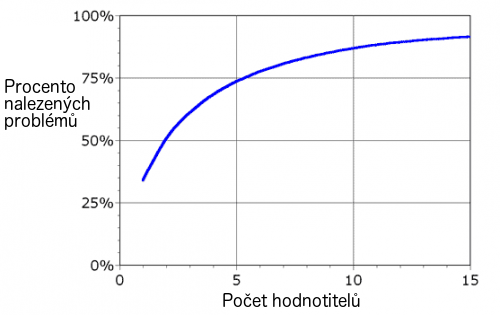
\includegraphics[width=0.99\textwidth]{./pictures/heur_eval_finding_curve_trans}
 \caption[Počet nalezených problémů v závislosti na počtu hodnotitelů]{Počet nalezených problémů v závislosti na počtu hodnotitelů. \cite{heur-eval-curve} (překlad vlastní)}\label{fig:heur}
\end{figure}

Po provedení heuristické analýzy byla vytvořena tabulka \ref{tab:heuristics} zobrazující nalezené problémy společně s jejich řešením a ohodnocením 1--5, kde číslo 1 identifikuje pouze drobný problém a číslo 5 velice závažný problém. Byla také vytvořena nová verze wireframe, která je také k nalezení v příloze této práce.

\begin{table}
\begin{tabular}{ c | c | p{9cm} }
Problém & Závažnost & Provedená úprava \\
\hline
1 & 3 & Při přidávání nového záznamu se bude měnit nadpis (title) podle toho zda je přidáván záznam o letu nebo ze simulátoru. \\
2 & 2 & Tlačítko \uv{Zavřít} bude přejmenováno na \uv{Zrušit}. Tato změna se týká obrazovek -- přidat záznam, přidat letadlo a přidat certifikát.\\
2 & 3 & U nastavení hledání bude tlačítko \uv{Zpět} přejmenováno na \uv{Zrušit}.\\
2 & 4 & Přejmenování záložky \uv{Nastavení} na \uv{Profil} a změnění ikonky.\\
2 & 4 & Přejmenování \uv{Můj profil} (v bývalé záložce \uv{Nastavení}) na \uv{Osobní informace}.\\
2 & 2 & Doplnění \uv{Certifikáty} na \uv{Zdravotní certifikáty}.\\
8 & 2 & U zobrazení všech záznamů jsou zredukovány zobrazené informace na datum, čas, místo a letadlo. \\
\end{tabular}
\caption[Nalezené problémy použitelnosti]{Nalezené problémy použitelnosti}\label{tab:heuristics}
\end{table}

\subsection{Uživatelské testy}
Uživatelské testy byly provedeny po heuristické analýze (na upraveném wireframe) ještě před samotnou implementací. Testy také nebylo možné provést v plné míře a sloužili převážné k odhalení nejvíce problematických částí návrhu uživatelského rozhraní.

Jakob Nielsen \cite{usabilityTestingNNG} doporučuje pět uživatelů na uživatelské testování. Však ze stejných důvodů jako u heuristické analýzy, byly zvoleni nyní pouze dva uživatelé.

Rozsáhlejší testování a heuristická analýza budou provedeny až po dokončení prototypu aplikace.

Testovaní uživatelé nebyly děleni v této fázi do skupin z důvodu jejich malého počtu. Podmínky na uživatele však kladeny byly -- oba uživatelé museli používat operační systém iOS minimálně po dobu jednoho rok a alespoň jeden z nich se musel pohybovat v leteckém průmyslu.

Pro oba uživatele byly vytvořeny stejné testovací scénáře. Uživateli, který neměl znalosti z letectví, byly nejprve vysvětleny základní pojmy nutné k absolvování scénářů a až poté bylo provedeno testování.

\subsubsection{Scénáře}
\begin{enumerate}
\item Právě jste dokončil svůj první let z Brna do Prahy. Z Brna jste odlétal v 7:00 a do Prahy jste přiletěl v 8:45, neměl jste žádné mezipřistání. Celou doby jste zastával funkci vedoucího pilota a letěl jste letadlem Boeing.
\item Zjistil jste, že jste u minulého záznamu chybně zaznamenal čas. Upravte tedy čas příletu do Prahy na 7:45.
\item Chcete si přidat další záznam, tentokrát z výcvikového zařízení. Zadejte dnešní datum, čas na zařízení dvě hodiny a znovu jste zastával funkci vedoucího pilota.
\item Aplikaci používáte již delší dobu a máte tedy i více záznamu. Zobrazte si pouze lety, které byly provedeny za poslední týden.
\item Jeden ze záznamů z minulého kroku smažte.
\item Zobrazte si svůj profil a zkontrolujte, zda jsou všechny položky vyplněny správně. Pokud ne, opravte chybně vyplněné nebo chybějící pole.
\item U letadla Boeing z prvního kroku chcete změnit model. Proveďte tuto úpravu.
\item Za poslední tři týdny jste absolvoval mnoho letů, zkontrolujte, zda jste nepřekročil jeden z limitů.
\item Dnes Vám vydali zdravotní certifikát třídy jedna (Class 1). Vložte ho do aplikace.
\item Vytvořte report ze všech záznamů letů i záznamů z výcvikového zařízení za posledních čtrnáct dní.
\end{enumerate}

\subsubsection{Výsledky testů a provedené úpravy}
Testovaní uživatelé byli při jednotlivých testech pozorováni, aby bylo zjištěno co a proč dělají špatně. Z čehož byly následně vyvozeny nutné úpravy v uživatelském rozhraní.

\begin{enumerate}
\item Smazání záznamu budu možné nyní ještě u detailu tohoto záznamu. Tato funkcionalita bude ještě znovu podrobena testu u prototypu aplikace. Gesto $swipe$ se u wireframe špatně testuje.
\item \uv{Má letadla} již nebudou pod záložkou \uv{Profil}, ale budou představovat samostatný $tab$.
\item Vytvoření reportu bude nyní označeno ještě navíc textem.
\item Při přidávání nového záznamu si uživatel nejprve vybere zda se jedná o záznam letu nebo o záznam ze simulátoru.
\item U zobrazení seznamu záznamů budou informace o jednotlivých záznamech v jiném pořadí -- datum, čas, místa vzletu a příletu a letadlo.
\end{enumerate}

Po provedení testování s pilotem byla diskutována navržená funkcionalita. Výsledkem této diskuze bylo:
\begin{itemize}
\item přidání celkové statistiky nalétaných hodin,
\item filtrování bude nyní možné i podle typu letadla,
\item záznamy letů budou zobrazovat nyní registrační číslo letadla místo jeho modelu, typu a varianty.
\end{itemize}

Případy užití zobrazené v této práci již zahrnují tuto přidanou a upravenou funkcionalitu. Po uživatelských testech a diskuzi byla i vytvořena poslední verze wireframe, také k nalezení v příloze této diplomové práce.

\section{Navržená řešení pro tvorbu aplikace}
Tato kapitola popisuje a zdůvodňuje zvolená řešení architektury, perzistence dat a FRP framework.

\subsection{Architektura}
Pro svou práci jsem si na základě navržených funkcionalit zvolil architekturu MVVM. Architektura MVVM eliminuje nevýhodu MVC -- příliš mnoho logiky a kódu ve vrstvě $Controller$, a na druhou stranu není zbytečně složitá (pro navrhovanou funkcionalitu) jako VIPER.

\subsection{Perzistence dat}
Pro tvorbu aplikace na evidenci letů jsem si zvolil možnost perzistence dat pomocí Realm. Prvním z důvodů této volby je podpora online i offline uložení dat. To umožňuje uživateli mít stejná data na více zařízeních, však i společně s možností používat aplikaci offline. Dalším důvodem bylo to, že je Realm zcela zdarma, což mu dává výhodu oproti iCloud -- Apple řešení.

\subsection{FRP framework}


\chapter{Realizace}
\label{chap:realizace}

\section{iOS aplikace a Swift}
\section{Unit testy}
\section{Použité nástroje při vývoji}
\section{Uživatelské testování}

\section{Postupy FRP v aplikaci}
\section{Zhodnocení MVVM a FRP}

\begin{conclusion}
	%sem napište závěr Vaší práce
\end{conclusion}

\bibliographystyle{csn690}
\bibliography{mybibliographyfile}

\appendix

\chapter{Seznam použitých zkratek}
% \printglossaries
\begin{description}
	\item[FRP] Funkcionálně reaktivní programování
	\item[MVC] Model View Controller
	\item[MVVM] Model View ViewModel
	\item[VIPER] View Interactor Presenter Entity Router
	\item[PC] Personal Computer
	\item[EASA] European Aviation Safety Agency
	\item[PIC] Pilot-in-command
	\item[SE] Single engine
	\item[ME] Multi engine
	\item[SPIC] Student PIC
	\item[PICUS] PIC under supervision
	\item[FSTD] flight simulation training devices
	\item[FI] Flight instructor
	\item[FE] Flight examiner
	\item[LAPL] Light Aircraft Pilot Licence
	\item[SPL] Sailplane Pilot Licence
	\item[BPL] Balloon Pilot Licence
	\item[PPL] Private Pilot Licence
\end{description}


% % % % % % % % % % % % % % % % % % % % % % % % % % % % 
% % Tuto kapitolu z výsledné práce ODSTRAŇTE.
% % % % % % % % % % % % % % % % % % % % % % % % % % % % 
% 
% \chapter{Návod k~použití této šablony}
% 
% Tento dokument slouží jako základ pro napsání závěrečné práce na Fakultě informačních technologií ČVUT v~Praze.
% 
% \section{Výběr základu}
% 
% Vyberte si šablonu podle druhu práce (bakalářská, diplomová), jazyka (čeština, angličtina) a kódování (ASCII, \mbox{UTF-8}, \mbox{ISO-8859-2} neboli latin2 a nebo \mbox{Windows-1250}). 
% 
% V~české variantě naleznete šablony v~souborech pojmenovaných ve formátu práce\_kódování.tex. Typ může být:
% \begin{description}
% 	\item[BP] bakalářská práce,
% 	\item[DP] diplomová (magisterská) práce.
% \end{description}
% Kódování, ve kterém chcete psát, může být:
% \begin{description}
% 	\item[UTF-8] kódování Unicode,
% 	\item[ISO-8859-2] latin2,
% 	\item[Windows-1250] znaková sada 1250 Windows.
% \end{description}
% V~případě nejistoty ohledně kódování doporučujeme následující postup:
% \begin{enumerate}
% 	\item Otevřete šablony pro kódování UTF-8 v~editoru prostého textu, který chcete pro psaní práce použít -- pokud můžete texty s~diakritikou normálně přečíst, použijte tuto šablonu.
% 	\item V~opačném případě postupujte dále podle toho, jaký operační systém používáte:
% 	\begin{itemize}
% 		\item v~případě Windows použijte šablonu pro kódování \mbox{Windows-1250},
% 		\item jinak zkuste použít šablonu pro kódování \mbox{ISO-8859-2}.
% 	\end{itemize}
% \end{enumerate}
% 
% 
% V~anglické variantě jsou šablony pojmenované podle typu práce, možnosti jsou:
% \begin{description}
% 	\item[bachelors] bakalářská práce,
% 	\item[masters] diplomová (magisterská) práce.
% \end{description}
% 
% \section{Použití šablony}
% 
% Šablona je určena pro zpracování systémem \LaTeXe{}. Text je možné psát v~textovém editoru jako prostý text, lze však také využít specializovaný editor pro \LaTeX{}, např. Kile.
% 
% Pro získání tisknutelného výstupu z~takto vytvořeného souboru použijte příkaz \verb|pdflatex|, kterému předáte cestu k~souboru jako parametr. Vhodný editor pro \LaTeX{} toto udělá za Vás. \verb|pdfcslatex| ani \verb|cslatex| \emph{nebudou} s~těmito šablonami fungovat.
% 
% Více informací o~použití systému \LaTeX{} najdete např. v~\cite{wikilatex}.
% 
% \subsection{Typografie}
% 
% Při psaní dodržujte typografické konvence zvoleného jazyka. České \uv{uvozovky} zapisujte použitím příkazu \verb|\uv|, kterému v~parametru předáte text, jenž má být v~uvozovkách. Anglické otevírací uvozovky se v~\LaTeX{}u zadávají jako dva zpětné apostrofy, uzavírací uvozovky jako dva apostrofy. Často chybně uváděný symbol "{} (palce) nemá s~uvozovkami nic společného.
% 
% Dále je třeba zabránit zalomení řádky mezi některými slovy, v~češtině např. za jednopísmennými předložkami a spojkami (vyjma \uv{a}). To docílíte vložením pružné nezalomitelné mezery -- znakem \texttt{\textasciitilde}. V~tomto případě to není třeba dělat ručně, lze použít program \verb|vlna|.
% 
%Více o~typografii viz \cite{kobltypo}.
% 
% \subsection{Obrázky}
% 
% Pro umožnění vkládání obrázků je vhodné použít balíček \verb|graphicx|, samotné vložení se provede příkazem \verb|\includegraphics|. Takto je možné vkládat obrázky ve formátu PDF, PNG a JPEG jestliže používáte pdf\LaTeX{} nebo ve formátu EPS jestliže používáte \LaTeX{}. Doporučujeme preferovat vektorové obrázky před rastrovými (vyjma fotografií).
% 
% \subsubsection{Získání vhodného formátu}
% 
% Pro získání vektorových formátů PDF nebo EPS z~jiných lze použít některý z~vektorových grafických editorů. Pro převod rastrového obrázku na vektorový lze použít rasterizaci, kterou mnohé editory zvládají (např. Inkscape). Pro konverze lze použít též nástroje pro dávkové zpracování běžně dodávané s~\LaTeX{}em, např. \verb|epstopdf|.
% 
% \subsubsection{Plovoucí prostředí}
% 
% Příkazem \verb|\includegraphics| lze obrázky vkládat přímo, doporučujeme však použít plovoucí prostředí, konkrétně \verb|figure|. Například obrázek \ref{fig:float} byl vložen tímto způsobem. Vůbec přitom nevadí, když je obrázek umístěn jinde, než bylo původně zamýšleno -- je tomu tak hlavně kvůli dodržení typografických konvencí. Namísto vynucování konkrétní pozice obrázku doporučujeme používat odkazování z~textu (dvojice příkazů \verb|\label| a \verb|\ref|).
% 
% \begin{figure}\centering
% 	
\includegraphics[width=0.5\textwidth, angle=30]{cvut-logo-bw}
% 	\caption[Příklad obrázku]{Ukázkový obrázek v~plovoucím prostředí}\label{fig:float}
% \end{figure}
% 
% \subsubsection{Verze obrázků}
% 
% % Gnuplot BW i barevně
% Může se hodit mít více verzí stejného obrázku, např. pro barevný či černobílý tisk a nebo pro prezentaci. S~pomocí některých nástrojů na generování grafiky je to snadné.
% 
% Máte-li například graf vytvořený v programu Gnuplot, můžete jeho černobílou variantu (viz obr. \ref{fig:gnuplot-bw}) vytvořit parametrem \verb|monochrome dashed| příkazu \verb|set term|. Barevnou variantu (viz obr. \ref{fig:gnuplot-col}) vhodnou na prezentace lze vytvořit parametrem \verb|colour solid|.
% 
% \begin{figure}\centering
% 	\includegraphics{gnuplot-bw}
% 	\caption{Černobílá varianta obrázku generovaného programem Gnuplot}\label{fig:gnuplot-bw}
% \end{figure}
% 
% \begin{figure}\centering
% 	\includegraphics{gnuplot-col}
% 	\caption{Barevná varianta obrázku generovaného programem Gnuplot}\label{fig:gnuplot-col}
% \end{figure}
% 
% 
% \subsection{Tabulky}
% 
% Tabulky lze zadávat různě, např. v~prostředí \verb|tabular|, avšak pro jejich vkládání platí to samé, co pro obrázky -- použijte plovoucí prostředí, v~tomto případě \verb|table|. Například tabulka \ref{tab:matematika} byla vložena tímto způsobem.
% 
% \begin{table}\centering
% 	\caption[Příklad tabulky]{Zadávání matematiky}\label{tab:matematika}
% 	\begin{tabular}{|l|l|c|c|}\hline
% 		Typ		& Prostředí		& \LaTeX{}ovská zkratka	& \TeX{}ovská zkratka	\tabularnewline \hline \hline
% 		Text		& \verb|math|		& \verb|\(...\)|	& \verb|$...$|		\tabularnewline \hline
% 		Displayed	& \verb|displaymath|	& \verb|\[...\]|	& \verb|$$...$$|	\tabularnewline \hline
% 	\end{tabular}
% \end{table}
% 
% % % % % % % % % % % % % % % % % % % % % % % % % % % % 

\chapter{Obsah přiloženého CD}

%upravte podle skutecnosti

\begin{figure}
	\dirtree{%
		.1 readme.txt\DTcomment{stručný popis obsahu CD}.
		.1 exe\DTcomment{adresář se spustitelnou formou implementace}.
		.1 src.
		.2 impl\DTcomment{zdrojové kódy implementace}.
		.2 thesis\DTcomment{zdrojová forma práce ve formátu \LaTeX{}}.
		.1 text\DTcomment{text práce}.
		.2 thesis.pdf\DTcomment{text práce ve formátu PDF}.
		.2 thesis.ps\DTcomment{text práce ve formátu PS}.
	}
\end{figure}

\end{document}
